\section{Exercise 1: Haar-like features and classification}

\subsection{Compute and visualize Haar-like features}

{\noindent\bfseries
Question 1:
\begin{itemize}
\item Explain the obtained 2-dimensional plot on the feature space.
\item Given this 2-dimensional plot, can we infer the defined Haar-like features are appropriate for face/non-face discrimination?
\end{itemize}}


Since we have just two features, each of the data points can be represented in a plane. The scatter plot can be found in figure \ref{fig:featscatter}. Moreover in figure \ref{fig:facesandnonfaceshighlighted} we show the square regions from which these features have been extracted. The first observation is that the positive and negative examples are not linearly separable, so this is not a trivial classification task. It turns out that the negative examples are more or less distributed along a vertical line while the positive examples, although somewhat more scattered, follow a horizontal trend. The neighbourhood around the intersection point between the two trends (approximately $ ( F_1, F_2) = ( 2.5 \cdot 10^3, 4 \cdot 10^4 ) $) seems like it is going to be troublesome when we get to classify new data.

\begin{figure}[h!tb]
	\centering
		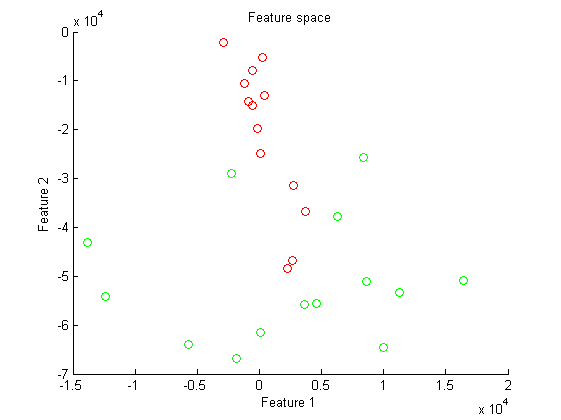
\includegraphics[width=0.6 \textwidth]{./img/ex1/featscatter.png}
	\caption{Scatter plot of the features for faces and non-faces}
	\label{fig:featscatter}
\end{figure}

\begin{figure}[h!tb]
	\centering
		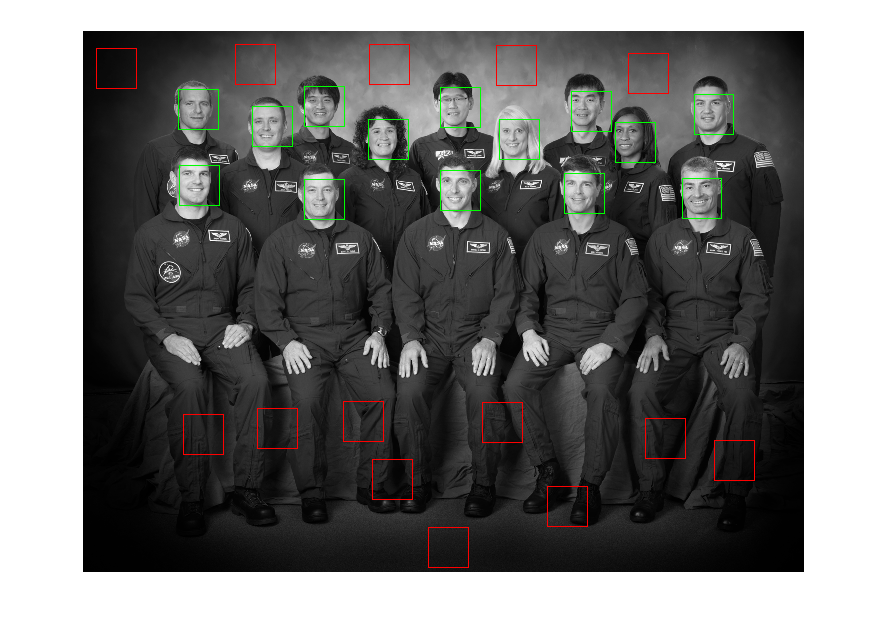
\includegraphics[width=\textwidth]{./img/ex1/facesandnonfaceshighlighted.png}
	\caption{Highlighted faces \& non-faces}
	\label{fig:facesandnonfaceshighlighted}
\end{figure}

These two features can be useful to discriminate between clear faces and clear foreground. However they cannot be relied upon when it comes to serious face detection and that is the very reason why more sophisticated face detection techniques like the one proposed by Viola \& Jones exist.


\subsection{Classification in the feature space}

{\noindent\bfseries Question 2: \\ \indent $ \bullet $ Is the result good enough? Explain your response}

The highlighted rectangles can be seen in figure \ref{fig:testfaceshighlighted}. Clearly there are some errors. We can see that there are 36 data rectangles and 23 of them have been correctly classified. Therefore, the predictive accuracy in this reduced test set is about $ 63.9 \% $, which is not a very appealing result.

\begin{figure}[h!tb]
	\centering
		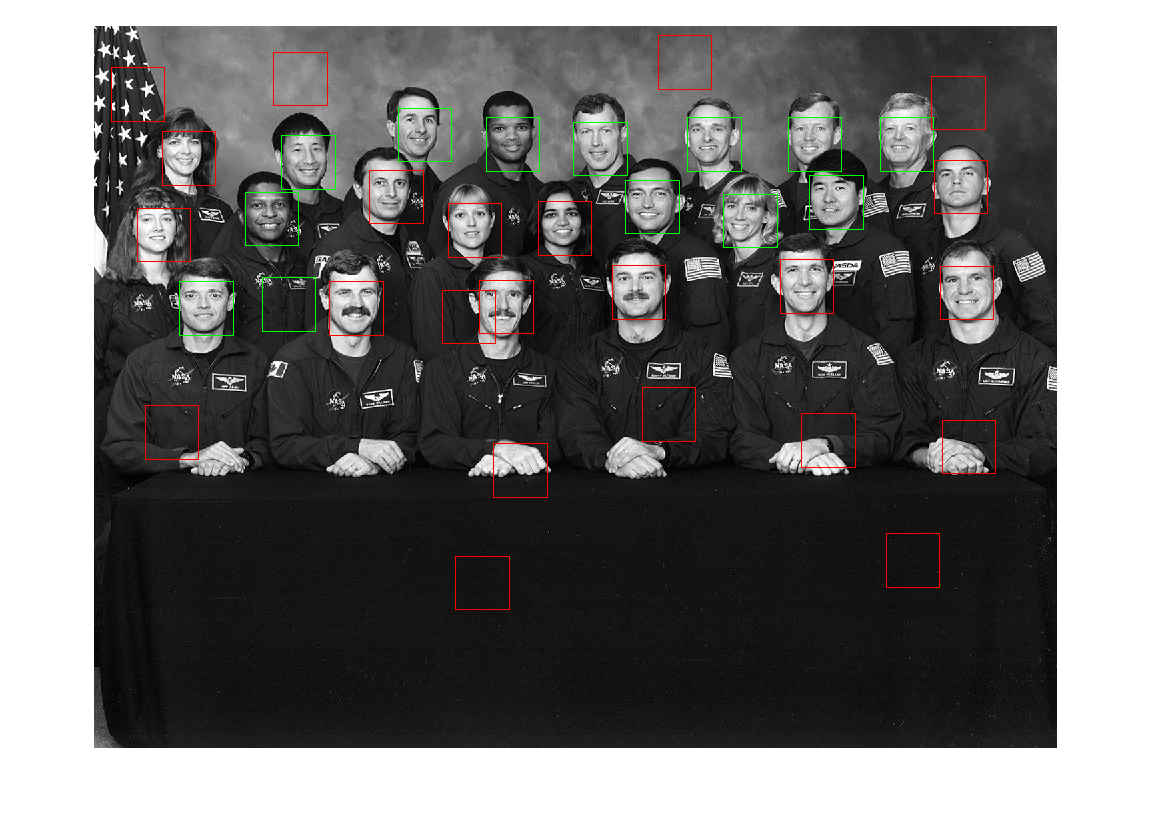
\includegraphics[width=\textwidth]{./img/ex1/testfaceshighlighted.png}
	\caption{Highlighted faces \& non-faces (test set)}
	\label{fig:testfaceshighlighted}
\end{figure}

For the sake of giving a more detailed conclusion, we have analysed the numbers with a bit more of depth. Table \ref{tab:comparisonrealdetected} shows the number of true/false positives/negatives. From these numbers we infer that the precision of the classifier in the test set ($ TP / ( TP + FP ) $) is about $ 92.3 \% $, while the recall ($ TP / ( TP + FN ) $) is $ 52.2 \% $. In more intuitive terms, this means that if the classifier is biased towards classifying an example as a negative one and that once it classifies a rectangle as a face, the probability that it is effectively a face is very high. We can see this noticing that many faces are misclassified as non-faces, while there is just a single non-face that is classified as a positive example.

In any case, the accuracy of the model is very low to consider it in a serious application.

\begin{table}[]
	\centering
	\begin{tabular}{lllll}
		           & \textbf{Detected P} & \textbf{Detected N} &  &  \\
		\textbf{Real P} & 12         & 11         &  &  \\
		\textbf{Real N} & 1          & 12         &  &  \\
	           &            &            &  & 
	\end{tabular}
	\caption{Ascertained label vs real one}
	\label{tab:comparisonrealdetected}
\end{table}

{\noindent\bfseries Question 3: \\ \indent $ \bullet $ What do you infer from the figure? Explain your response}

The scatter plot is shown in figure \ref{fig:feattestscatter}. Our previous observation is more or less coherent which this new plot (if only the negative examples are more of a round cluster now, instead of a line). The first thing we can observe is that the negative examples are more densely packed than the positive ones, which lie more scattered and are distributed with a greater variance. Thanks to this the classifier has been able to correctly detect as faces the points located far from the ``center of mass''. On the other hand, we can see that the points that are in the middle of the plot and that are classified as negative examples probably correspond to the badly classified faces. This is just as we have foreseen in the former section of this document.

\begin{figure}[h!tb]
	\centering
		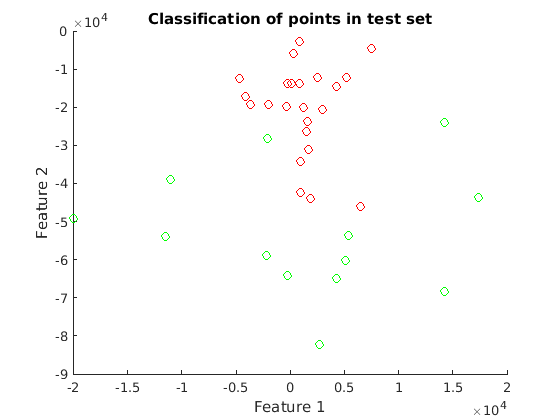
\includegraphics[width=0.6 \textwidth]{./img/ex1/feattestscatter.png}
	\caption{Highlighted faces \& non-faces (test set)}
	\label{fig:feattestscatter}
\end{figure}